
\documentclass[16pt,a4paper]{article}
\usepackage[utf8]{inputenc}
\usepackage{amsmath}
\usepackage{amsfonts}
\usepackage{amssymb}
\usepackage{amsthm}
\usepackage{tikz-cd}

\usetikzlibrary{matrix}
\usepackage[many]{tcolorbox}
\tcbuselibrary{skins,breakable}


\newtcbtheorem{defn}{Definition}{
    width=\textwidth,
    colback=white!20,
    colframe=orange,
    colbacktitle=orange,
    fonttitle=\bfseries,
    sharp corners,
    boxrule=1pt,
    breakable,
    enhanced,
    boxed title style={sharp corners},
    attach boxed title to top left
}{def}


\newtcbtheorem{axm}{Axiom}{
    width=\textwidth,
    colback=white!20,
    colframe=black,
    colbacktitle=black,
    fonttitle=\bfseries,
    sharp corners,
    boxrule=1pt,
    breakable,
    enhanced jigsaw,
    boxed title style={sharp corners},
    attach boxed title to top left
}{axm}


\newtcbtheorem{thm}{Theorem}{
    width=\textwidth,
    colback=deepblue!2,
    colframe=deepblue,
    colbacktitle=deepblue,
    fonttitle=\bfseries,
    sharp corners,
    boxrule=1pt,
    breakable,
    enhanced,
    boxed title style={sharp corners},
    attach boxed title to top left
}{thm}

\newtcbtheorem{lemm}{Lemma}{
    width=\textwidth,
    colback=deepred!0,
    colframe=deepred,
    colbacktitle=deepred,
    fonttitle=\bfseries,
    sharp corners,
    boxrule=1pt,
    breakable,
    enhanced,
    boxed title style={sharp corners},
    attach boxed title to top left
}{lemm}



\newtcbtheorem{coll}{Corollary}{
    width=\textwidth,
    colback=white!20,
    colframe=gray,
    colbacktitle=gray,
    fonttitle=\bfseries,
    sharp corners,
    boxrule=1pt,
    breakable,
    enhanced,
    boxed title style={sharp corners},
    attach boxed title to top left
}{coll}


\usepackage[pdftex,breaklinks,colorlinks,
citecolor=blue,
urlcolor=blue,
pdftitle={Math 145 notes},
pdfauthor={Thaqib},
pdfsubject={Math 145}]{hyperref}



\usepackage{setspace}
\setstretch{1.7}
\usepackage{graphicx}
\usepackage[left=2cm,right=2cm,top=2cm,bottom=2cm]{geometry}

\usepackage{listings}
\usepackage{color}
\definecolor{dkgreen}{rgb}{0,0.6,0}
\definecolor{gray}{rgb}{0.5,0.5,0.5}
\definecolor{mauve}{rgb}{0.58,0,0.82}

\definecolor{deepblue}{rgb}{0,0,0.5}
\definecolor{deepred}{rgb}{0.6,0,0}
\definecolor{deepgreen}{rgb}{0,0.5,0}
\lstset{frame=tb,
  language=python,
  aboveskip=2mm,
  belowskip=2mm,
  showstringspaces=false,
  columns=flexible,
  basicstyle={\linespread{0.9}\small	tfamily},
  numbers=none,
  numberstyle=	iny\color{gray},
  keywordstyle=\color{blue},
  commentstyle=\color{dkgreen},
  stringstyle=\color{deepred},
  breaklines=true,
  breakatwhitespace=true,
  tabsize=4
}

\theoremstyle{definition}
\newtheorem{definition}{Definition}[section]

\newtheorem{theorem}{Theorem}[section]
\newtheorem{corollary}{Corollary}[theorem]
\newtheorem{lemma}[theorem]{Lemma}
\tikzstyle{vertex}=[shape=circle, minimum size=2mm, inner sep=0, fill]
\tikzstyle{opendot}=[shape=circle, minimum size=2mm, inner sep=0, fill=white, draw]
\newcommand{\axis}[2]{\draw[help lines, <->] (-#1,0)--(#1,0) node[right]{$x$};
\draw[help lines, <->] (0,-#2)--(0,#2) node[above]{$y$};}
\newcommand{\aaxis}[4]{\draw[help lines, <->] (-#1,0)--(#2,0) 
node[right]{$x$};
\draw[help lines, <->] (0,-#3)--(0,#4) node[above]{$y$};}

\newcommand{\OR}{\vee}

\newcommand{\AND}{\wedge}

\author{Thaqib Mo.}
\title{ Reading-14 }
\begin{document}
\maketitle
\newpage
\section{Comparing Cardinalities of Sets}

\begin{defn}{Cardinality}{}
2 sets have the same \textit{cardinality} if there is a bijection $f:A\rightarrow B$. We write $|A| = |B|$ to indicate this. 
\end{defn}
This relation forms an equivalence relation. Shown in A04, so the equivalence relation $\mathcal{R}$ is given by:
\[A\mathcal{R}B \text{ if there is a bijection $f:A\rightarrow B$}\]


\begin{defn}{Comparing cardinality}{}
If we have 2 sets $A$ , $B$ we say that the cardinality of $A$ is less than or equal to $|B|$, then we write $|A|\leq |B|$, if there is an injective function $f:A\rightarrow B$
\end{defn}

\subsection{Properties of cardinality $\leq$}

We want to prove that the $\leq$ relation behaves as an order relation. This requires some lemmas to be proven before the actual proof. 

\begin{lemm}{}{}
Suppose we have $A_1, B, A$ such that $A_1 \subseteq B \subseteq A$. If $|A_1| = |A|$ then $|B| = |A|$
\end{lemm}{}{}

\begin{proof}
The goal is to create a bijection $g:A\rightarrow B$. \\

As we are given $|A_1| = |A|$ so let $f:A  \rightarrow A_1$ be a bijection. Now we use $f$ to define a sequence of sets.  We set $A_0 = A$ and $B_0 = B$ and for each $n \in \mathbb{N}$ we set:

\[A_{n+1} = f(A_n)\quad B_{n+1} = f(B_n)\] 

Since $f$ is bijection from $A$ to $A_1$ we have $f(A_0) = A_1$. For each $n\in \mathbb{N}$ we can say $A_{n+1} \subseteq A_n$. This can be proven with induction as we already know that $A_1 \subseteq A_0$.   \\

To define the bijection $g:A\rightarrow B$, it will map all elements of $A\setminus B$ to $B$ but we need elements in $B$ to map them to.  To get this we define: 
\[C_n = A_n \setminus B_n\]
and the set 
\[C = \bigcup_{n=0}^{\infty}C_n\]
\newpage
We claim that $f(C_n) = C_{n+1}$. First note that if $a\in f(C_n)$, then $a= f(c)$ for some $c\in C_n$. By definition $c \in A_n$ and $c\notin B_n$. Then $f(c) \in f(A_n) = A_{n+1}$. We also have $f(c) \notin f(B_n)$. If we have $f(c) = f(b)$ for some $b\in B_n$ as $f$ is bijection we must have $c =b$ that means we have $c\in B_n$ which is a contradiction.\\

So now we have $f(c) \in A_{n+1}\setminus B_{n+1}$ that is $f(c) \in C_{n+1}$, this proves that $f(C_n) \subseteq C_{n+1}$. Now assume we have $a\in C_{n+1}$, then $c\in A_{n+1}$ and $a\notin B_{n+1}$. This leads to $a = f(a^\prime)$ for some $a^\prime \in A_n$, since $a\notin B_{n+1}$ this means that $a^\prime \in B_n $. This means that $a^\prime \in C_n$ so that $a = f(a^\prime) \in f(C_n)$. This proves $C_{n+1} \subseteq f(C_n)$. Therefore we have $f(C_n) = C_{n+1}$. 
\\ 

The next claim is 
\[f(C) = \bigcup_{n=1}^{\infty}C_n \]

Now assume we have $a \in f(C)$, then $a = f(c)$ for some $c \in C$ then $c \in C_n$ for some $n \in \mathbb{N}$. This means $a \in f(C) \in f(C_n) = C_{n+1}$ proving we have $a\in \bigcup_{n=1}^{\infty}C_n$.  Now if we have $a\in \bigcup_{n=1}^{\infty}C_n$ then $a \in C_n$ for some $n$. Then if we have $n-1 \in \mathbb{N}$ then we have $C_n = f(C_{n-1})$. So $a = f(c)$ for some $c \in C_{n-1}$ then we can write $a \in f(C)$. This proves the claim. 
\\

Finally, we define another set $D = A\setminus C$. We define our bijection $g$ by  defining it separately on the two sets $C$ and $D$. All the elements of $C$ are mapped to a smaller set and the elements of $D$ are left where they are. 

\[
g(x) = \begin{cases}
f(x) & \text{if $x \in C$}\\
x & \text{if $x \in D$}
\end{cases}
\]  
First we need to verify for all $x\in A$ we have $g(x) \in B$. If $x \in C$, then $f(x) \in C_n$ for some $n\geq 1$, which implies $f(x) \in A_n$. Now since $A_0 \supseteq A_1 \supseteq A_2 \cdots$. In particular that $f(x) \in A_1$. We have $f(x) \in A_1$ and $A_1 \subseteq B$, so $f(x) \in B$. Otherwise if $x \in D$, then $x \notin C$, in particular $x\notin C_0$ so we have $x\not in A\setminus B$ which means that it is \textbf{\textit{not the case }}that $x\notin B$, then whenever $x\in D$ we have $x\in D$. 

Now we need to show that $g$ is a bijection. To see that it's one-to-one let $x_1, x_2 \in A$ such that $g(x_1) = g(x_2)$. If $x_1$ and $x_2$ both belong to $C$ then $f(x_1) = f(x_2)$ then $x_1 = x_2$. If both belong to $D$ then we immediately have $x_1 = x_2$. If $x_1 \in C$ and $x_2 \in D$, then $f(x_1) = x_2$ but we must have $f(x_1) \in C$ so we have a contradiction. The same contradiction follows for $x_1 \in D$ and $x_2 \in C$. So we have shown $g$ is injective. \\

To prove $g$ is surjective, assume we are given $b\in B$. If $b\in f(C)$ then clearly there is $c\in C$ such that $f(c) = b$. Otherwise if $b\notin f(C)$. Then we can have $b \in C_0$ or $b \in D$. If $b \in C_0$ then $b\in A\setminus B$ but we already have $b\in B$ so this is a contradiction. Otherwise if we have $b\in D$ then $g(b) = b$ and we are done. 

In conclusion the function $g:A\rightarrow B$ is a bijection so by definition we get $|A|= |B|$ 
\end{proof}

\begin{thm}{properties of $\leq$}{}
\begin{itemize}
\item[(1)] For all sets $A, B, C$, if $|A|\leq |B|$ and $|A|=|C|$ then $|C|\leq |B|$ 

\item[(2)] For all sets $A, B, C$, if $|A|\leq |B|$ and $|B|=|C|$ then $|A|\leq |C|$

\item[(3)] For all sets $A, B, C$, if $|A|\leq |B|$ and $|B|\leq |C|$ then $|A|\leq |C|$

\item[(4)] (Cantor-Schroder-Bernstein Theorem)  For all sets $A$ $B$, if $|A|\leq |B|$ and $|B| \leq |A|$ then $|A| = |B|$
 
\end{itemize}
\end{thm}

\begin{proof}
The properties $(1), (2), (3)$ all follow from the same general fact if $f:A\rightarrow B$ and $gB \rightarrow C$ are both injective functions then so is $g\circ f: A\rightarrow C$
\\

To prove $(4)$ Cantor-Schroder-Bernstein theorem, suppose we have injective functions $f:A\rightarrow B$ and $g:B\rightarrow A$. Then the composition $g\circ f: A\rightarrow A$, which is also injective. \\
Now let $X = g(B)$ and $Y = g(f(A))$. Clearly $X\subset A$, and since $f(A)\subset B$, we get $f(A) \subset B$  so we get $Y \subset X$. Since $g\circ f$ is injective, it is also a bijective function function from $A$ to $Y$, we get $|A| = |Y|$. \\

So we have $Y\subseteq X \subseteq A$ and $|Y| = |A|$, applying \textit{Lemma 1} we can conclude $|A| = |X|$. But $X = g(B)$, and $g$ is injective, so $g:B\rightarrow X$ is a bijection and $|X| = |B|$ so we can conclude $|B| = |A|$


\end{proof}




\newpage
\section{Finite Sets}

\begin{defn}{Finite Sets}{}
A set is $A$ called \textit{finite} if $A$ has the same cardinality as $n$ for some $n\in \mathbb{N}$. We write $|A| = n$ and we say $A$ has $n$ elements. A set is infinite if it is not finite. 
\end{defn}

For a finite set we want to have the cardinality to be well defined. We cannot have $|A| = m$ and $|A| = n$ for distinct $m,n$. The following lemma rules out that possibility. 

\begin{lemm}{}{}
For any $n\in \mathbb{N}$, there is no injective mapping from $n$ to a proper subset of $X\subset n$. 
\end{lemm}
\begin{proof}
Assume this is not true. Then by the well ordering principle, we can find some least $n\in \mathbb{N}$ for which there is an injective mapping from $n$ to one of its proper sets. Clearly $n\neq 0$ because there are no proper subsets of 0.  Then there is no injective mapping from 0 to a proper subset of 0. 
\\

Now there are 2 cases: either $n-1\in X$ or $n-1\notin X$. If we have $n-1\notin X$ then $X\subseteq (n-1)$, and $n-1 \in \mathbb{N}$ because $n\neq 0$. If $f:n\rightarrow X$ is an injective mapping, then we can now define a new mapping $g:n-1 \rightarrow X\setminus \{f(n-1)\}$ by taking $g(k) = f(k)$ when every $k\in n-1$. Now $g$ is automatically an injection since $f$ is, and $g$ is mapping $n-1$ to a proper subset of $n-1$ since $X$ is a proper subset of $n-1$ since we know that $g$ atleast will mist $f(n-1)\in n-1$. This contradicts that $n$ was minimal. 
\\
Now suppose $n-1\in X$. Since $f$ is injective, we know that $n-1 = f(k)$ for some unique $k\in n$. We can use this to define a new function $g:n-1\rightarrow X\setminus \{n-1\}$ by taking: 

\[
g(i) = 
\begin{cases}
f(i) & \text{ if $i\neq k$}\\
f(n-1) & \text{ if $i = k$ } 
\end{cases}
\]
This function is same as $f$ but instead of $f(k)$ we map it to $f(n-1)$ to make sure that it maps into $X\setminus \{n-1\}$, $g$ is injective and maps $n-1$ to a proper subset of $n-1$. Again this contradicts that $n$ is minimal.   
\end{proof}

This lemma has the following consequences:

\begin{coll}{}{}
If $A$ is finite set such that $|A| = n$ and $|A| = m$ then $n=m$ for all $n,m\in \mathbb{N}$
\end{coll}
\begin{proof}
This implies that both $n$ and $m$ have the same cardinality. Assume that we have $n\neq m$. We have a bijection $f:n\rightarrow m$ if $n\neq m$ then either $n\subset m$ or $m\subset n$ in both cases we cannot have a bijection from $n$ to $m$ or the other way because of \textbf{Lemma 2} so this is a contradiction. 
\end{proof}



\newpage


Another consequence of \textbf{Lemma 2} is: 
\begin{thm}{}{}
The set $\mathbb{N}$ is infinite
\end{thm}

Consider the bijection $f:\mathbb{N} \rightarrow \mathbb{N}$ given by $d(n) = 2n$ this is a bijection so $\mathbb{N}$ is infinite, by definition as it maps $\mathbb{N}$ to a proper subset of $\mathbb{N}$. $\quad \qed$




\subsection{Properties of Finite sets}
\begin{thm}{Subsets of finite sets are finite}{}
If $A$ is a \textit{finite} set and $B\subseteq A$ then $|B|\leq |A|$ and $B$ is \textit{finite}
\end{thm}{}{}

\begin{proof}
We can define a function $\iota : B\rightarrow A$ by $\iota(b) = b$. Clearly this is an injective mapping so we have $|B|\leq |A|$. Now since we know that $A$ is finite we have $|A| = n$ for some $n\in \mathbb{N}$. For $n=0$ we already have that $B$ is finite. Consider $n\geq 1$ we can index the elements of $A$ since there is a bijection from $A$ to $n$, so we can write : 

\[A = \{a_0, a_1, \ldots, a_{n-1}\}\]



Given that $B$ is a subset of $A$ if $B$ is empty we are done. Otherwise, there is some least index $i$ for which $a_i \in B$. We call that $b_0$. If we have $B = \{b_0\}$ it is finite and we are done. Otherwise there is another index $i_1 > i$ for which $a_{i_1}\in B$ and $B= \{b_0, b_1\}$. If we keep repeating this process we must end at some point as $A$ is finite. So at the end we get a sequence of indices $i_0 < i_1 < i_2 < \ldots$ for which $a_{i_0}, a_{i_1}, a_{i,2}, \ldots \in B$. So for each element in $B$ in the form $a_{i_j}$ we can map it to $j$ creating a bijection from $B$ to a natural number. 
\end{proof}

Note: Every application of Axiom Schema of Comprehension leads to a subset of $X$. So if only finite sets are allowed to exist \textbf{Theorem 3} shows that Axiom of Comprehension can only derive more finite sets. 


\newpage

\section{Countable Sets}
\begin{defn}{Countable sets}{}
A set $A$ is called countable if $|A| = |\mathbb{N}|$, it is called \textit{most countable} if $|A|\leq |\mathbb{N}|$. If $|A|$ is countable, we write $A = \aleph_0$ 
\end{defn}
For any countable set we have a bijection from $A$ to $\mathbb{N}$ so we can list the elements as an infinite sequence  of $A = \{a_0, a_1, \ldots \}$ conversely if we can list the elements as an infinite sequence it is countable. 

\begin{lemm}{Subsets of countable sets}{} \label{lem3}
Every subset of a countable set are countable or finite
\end{lemm}
\begin{proof}
Suppose we have $A$ and $B\subseteq B$. If $B$ is finite we are done. So assume $B$ is infinite. We can write the elements of $A$ as a sequence $A = \{a_0, a_1, a_2, \ldots \}$  we can define elements of $B$ recursively. First choose the smallest index $k_0$ such that $a_{k_0} \in B$ then choose the next $k_1>k_0$ the continuing for each natural number $i$, we let $k_i > k_{i-1}$ such that $a_{k_i}\in B$ and taking $b_i = a_{k_i}$. We can do this because $B\setminus \{b_0, b_1, b_2, \ldots\}$ will always be non empty given that it is infinite. So we can enumerate the elements of $B$ as a subsequence of $\{a_n\}$ namely $\{a_{k_n}\}$  This proves that $B$ is countable. 
\end{proof}


\begin{lemm}{Cartesian Product of Countable sets}{}\label{lem4}
If $A$ and $B$ are countable then $A\times B$ is also countable.
\end{lemm}

\begin{figure}[hbtp]
\centering
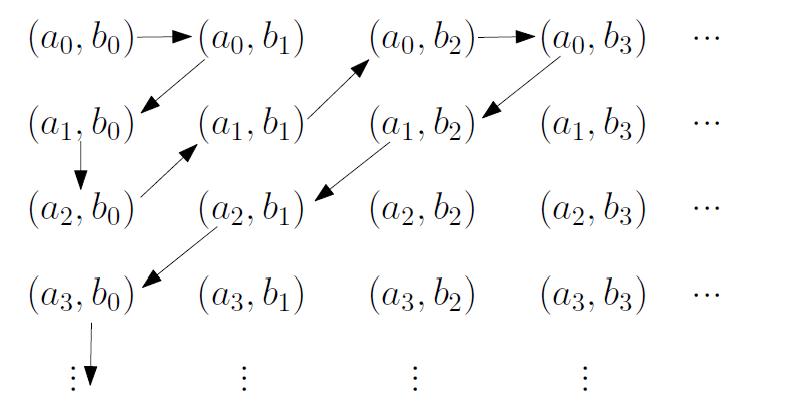
\includegraphics[scale=1]{figs/fig0.png}
\end{figure}
$\qquad\qquad\qquad\qquad\qquad\qquad\qquad\qquad\qquad\qquad\qquad\qquad\qquad\qquad\qquad\qquad\qquad\qed$



We can use induction to prove for finitely many countable sets $A_0, A_1, \ldots A_n$ the product $\prod\limits_{i=0}^nA_i$ is also finite. \\

These results can be used to show that $\mathbb{Q}$ is countable. We can write any number in the form $\frac{a}{b}$ so it can be represented as $(a,b)$ of integers where $b\neq 0$. We know that $\mathbb{Z\times Z}$ is countable. So we can treat $\mathbb{Q}$ as a subset of $\mathbb{Z\times Z}$. Every subset of a countable set is either countable or finite. $\mathbb{Q}$ contains the infinite set $\mathbb{Z}$ so $\mathbb{Q}$ is not finite therefore is is countable.  


\newpage	

\subsection{Building Sets from Countable Sets}
\begin{lemm}{Union of Countable sets}{}
Let $A, B$ countable sets then $A\cup B$ is countable. 
\end{lemm}
\begin{proof}
Since $A$, $B$ are both countable, let $A = \{a_n\}$ and $B = \{b_n\}$ we can define a sequence whose range is $A\cup B$, which we call $c_0, c_1, c_2, \ldots, $ by taking $c_{2k} = a_{k}$ and $c_{2k+1} = b_k$ for each $k\in \mathbb{N}$. The sequence $\{c_n\}$ might have some duplicates, after removing the duplicates we end up with a sequence $c_0, c_1, c_2, \ldots$ which enumerates $A\cup B$, this sequence has a bijection to one of it's proper subsets to it is infinite and \hyperref[lem3]{Lemma 3} shows that this is countable. 
\end{proof}

This can be extended to union of finite number of countable sets this can be proved using induction. So we have for the set: 

\[\bigcup_{i = 0}^n A_i \text{ Is countable}\]
To prove the case where we have a countable collection of countable sets. Consider: 

\[\mathcal{C} = \{A_0, A_1, A_2, \ldots\}\]
Here $\mathcal{C}$ is a countable collection of countable sets. We want to show that $\bigcup \mathcal{C}$ is also countable. Using axiom of choice we can enumerate all the countable sets at once. Let $A_i = \{a_{i,0}, a_{i,1}, a_{i,2}, \ldots\}$ for each $i \in \mathbb{N}$. Then similar to \hyperref[lem4]{Lemma 4} we can list $a_{0,0}$ first then $a_{1,0}$ then $a_{0,1}$ and continuing all the indices whose sum is 1 then 2 then 3 $\ldots$. This might have some duplicates, removing them and re indexing the sequence will yield the  union $\bigcup \mathcal{C}$ as enumerated by an infinite sequence. Thus union of countable collection of countable sets is countable. This yields the following theorem.  

\begin{thm}{Countable Union of Countable sets}{}
For a of a countable collection of countable sets $\mathcal{C} = \{A_0, A_1, A_2, \ldots,\}$ the union

\[
\bigcup_{i=0}^\infty A_i \text{ Is Countable}
\]

\end{thm} 



\newpage

\section{Uncountable Sets}

\subsection{The Real Numbers $\mathbb{R}$ are Uncountable}


\paragraph{Proposition:} $|(0,1)| = |\mathbb{R}|$
\begin{proof}
Consider the function  $f:(0,1) \rightarrow \mathbb{R}$ defined as:

\[f(x) = \frac{1-2x}{x(x-1)}\]
It can be shown that this function is both injective and surjective. Therefore this is a bijection, leading to $|(0,1)| = |\mathbb{R}|$
\end{proof}


\begin{thm}{$\mathbb{R}$ is uncountable}{}
The set of real numbers is uncountable
\end{thm}

\begin{proof}
We can try and enumerate all the real number between $(0,1)$ as all the numbers have a decimal expansion we can list with as

\begin{figure}[hbtp]
\centering
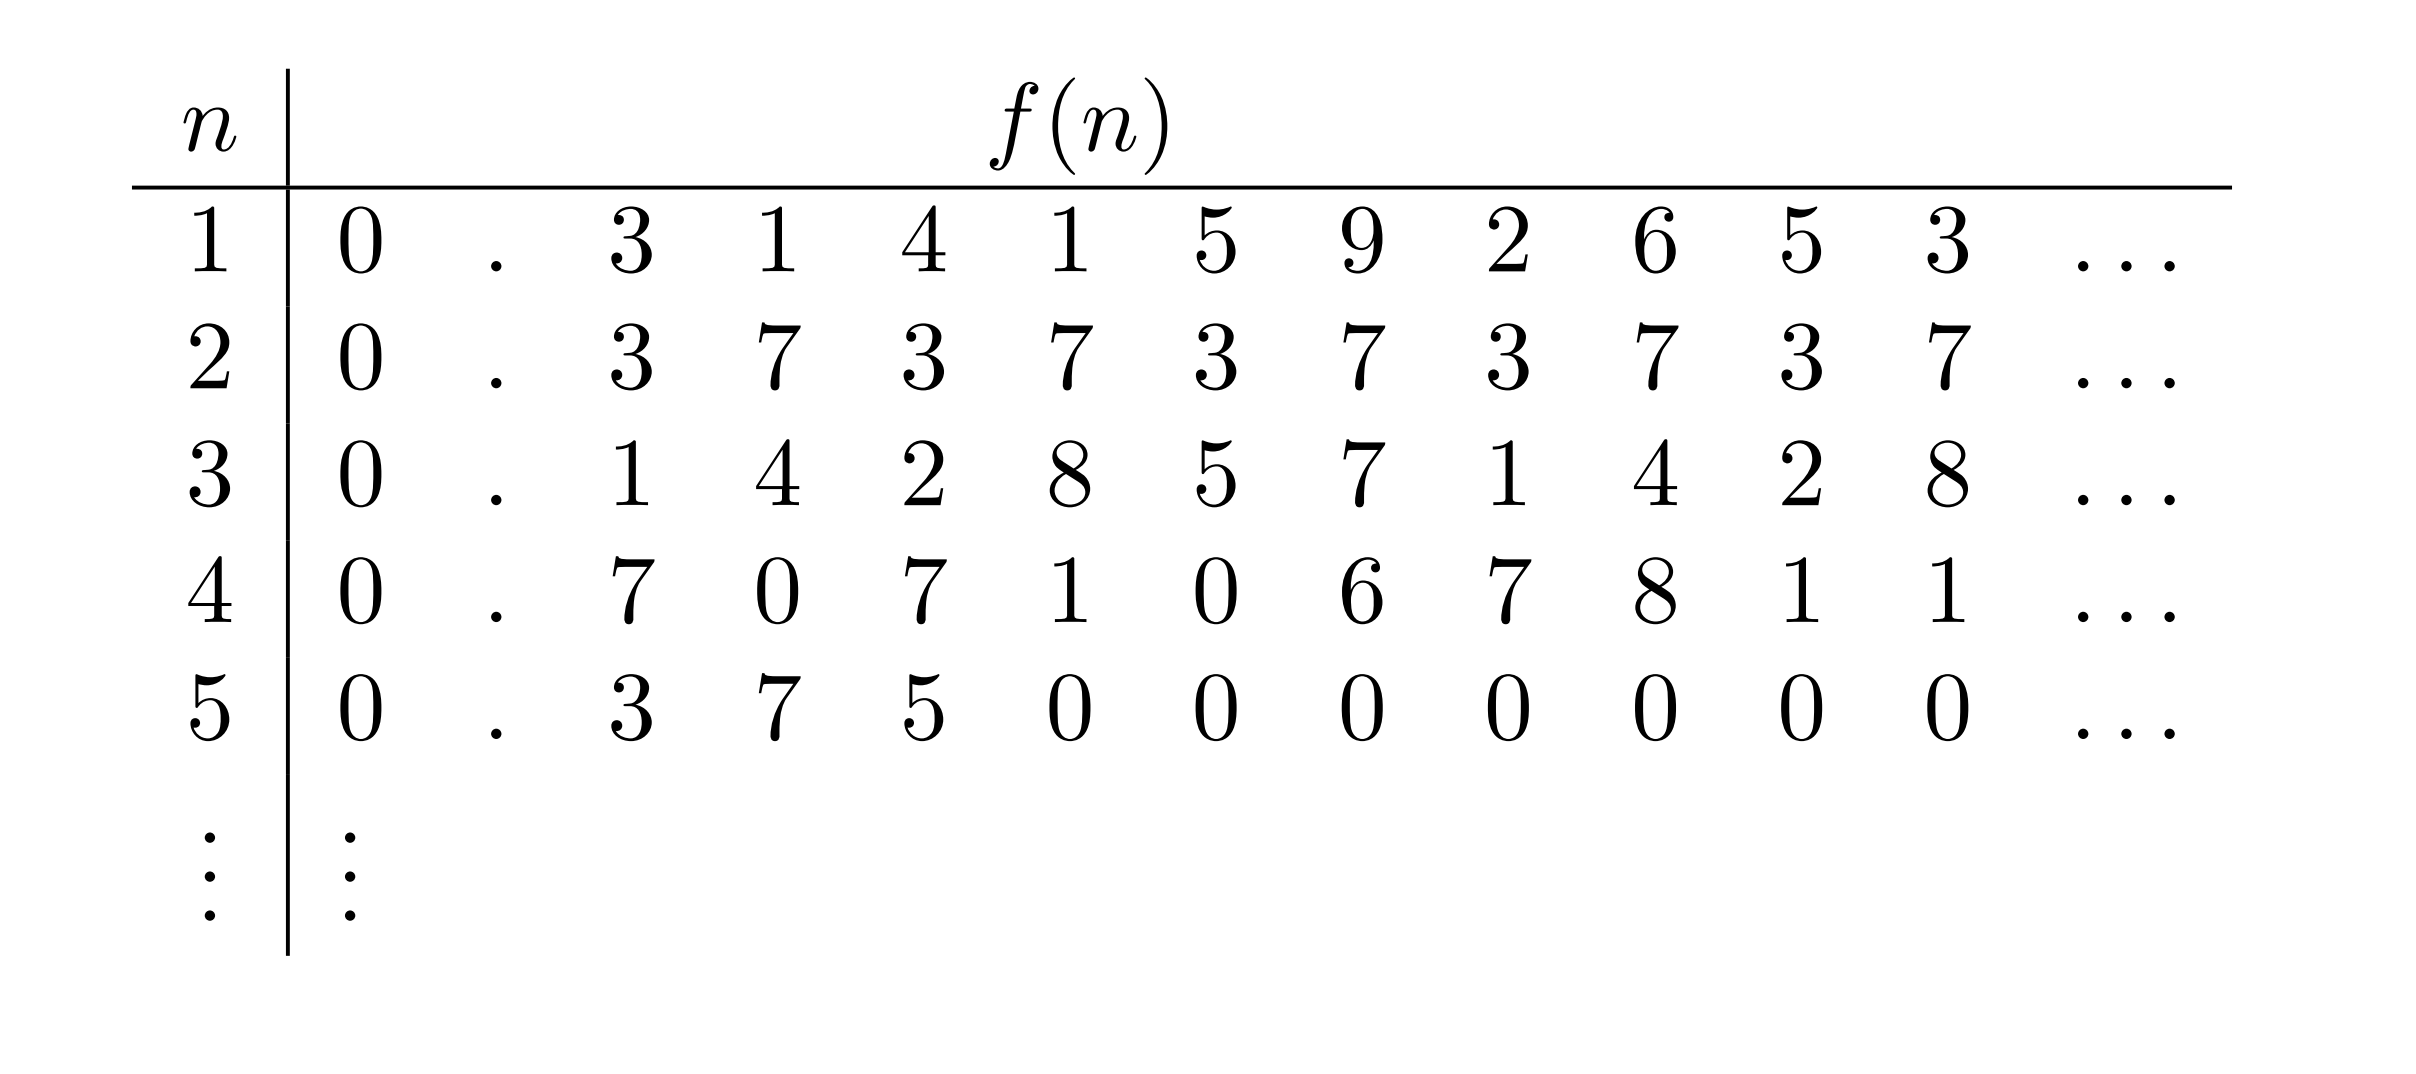
\includegraphics[scale=0.3]{figs/fig1.png}
\end{figure}
Now we can write the sequence as:

\begin{align*}
r_1 = 0.\boxed{b_{1,1}}b_{1,2}b_{1,3}b_{1,4}\ldots \\
r_2 = 0.b_{2,1}\boxed{b_{2,2}}b_{2,3}b_{2,4}\ldots \\
r_3 = 0.b_{3,1}{b_{3,2}}\boxed{b_{3,3}}b_{3,4}\ldots \\
r_4 = 0.b_{4,1}{b_{4,2}}b_{4,3}\boxed{b_{2,4}}\ldots \\
\vdots\;\;\;\;\;\;\qquad\qquad\qquad\;\;\ddots \quad
\end{align*}
Selecting the diagonals we can make a new number $r$ as 
\[r = 0.c_1 c_2 c_3 \ldots\] 
 For each $c_i$ we have $c_i = \begin{cases}
4 & \text{ If $b_{i,i} \neq 4$}\\
5 & \text{ If $b_{i,i} = 4$}\\
 \end{cases}$ we know that $r\in (0,1)$ but $r$ is not in the sequence $r_n$ since it differs at the $i^\text{th}$ decimal position for each $r_n$. So no matter how we try to enumerate $(0,1)$ we cannot do it. So $(0,1)$ is uncountable and so is $\mathbb{R}$ 
\end{proof} 


\begin{thm}{Power set of $\mathbb{N}$ and $\mathbb{R}$}{}
$|\mathcal{P}(\mathbb{N})| = |\mathbb{R}|$, $\mathcal{P}(\mathbb{N})$ is uncountable. 
\end{thm}






























































\end{document}
